% Brilliant documentation:
% http://mirror.ox.ac.uk/sites/ctan.org/macros/latex/contrib/beamer/doc/beameruserguide.pdf

\usepackage{beamerthemesplit}
\usepackage{tikz}
\usetikzlibrary{arrows.meta,shapes,backgrounds,positioning,shapes.multipart}
\usepackage{textpos} 
\usepackage{hyperref}
\usepackage{graphicx}
\usepackage{calc}
%\usepackage{listings}
%\usepackage[usenames,dvipsnames,svgnames,table]{xcolor} PACKAGE CLASH!
%\usepackage{color}
\newlength{\popupimagewidth}

\setlength{\popupimagewidth}{\textwidth*3/5}
\setcounter{tocdepth}{2}% Don't show subsubsections in table of contents

\addtobeamertemplate{frametitle}{}{
  % From http://tex.stackexchange.com/a/180628
  \begin{textblock*}{100mm}(\textwidth,-1cm)
    
\includegraphics[height=1cm,width=1cm]{ise-logo.jpg}
  \end{textblock*}
}

%\newcommand{\defineterm}[2]{#1 -- #2}
\newcommand{\articleheading}[1]{\subsubsection{#1}}

\title{Linked Open Data in Action}
\author{Matt Wallis}
\date{\today}
\date{February 17, 2017}

% From http://tex.stackexchange.com/a/183966:
\tikzset{
    invisible/.style={opacity=0,text opacity=0},
    visible on/.style={alt=#1{}{invisible}},
    alt/.code args={<#1>#2#3}{%
      \alt<#1>{\pgfkeysalso{#2}}{\pgfkeysalso{#3}} % \pgfkeysalso doesn't change the path
    },
}

\begin{document}
\maketitle
This is a handout to accompany the presentation at the Open:2017 conference.
It contains all of the slides, and additional notes too.

\frame{
  \begin{center}
    Download handout now

    http://

    Twitter: \href{https://twitter.com/SolidarityEcon}{@SolidarityEcon}
  \end{center}
}
\frame{\titlepage}

\frame{\tableofcontents}

\section{Institute for Solidarity Economics}
\frame
{
  \frametitle{Institute for Solidarity Economics}
  \begin{center}
    
\includegraphics[height=2cm,width=2cm]{ise-logo.jpg}
  \end{center}
  \begin{itemize}
    \item<1-> \url{http://solidarityeconomics.org}
    \item<1-> The Solidarity Economy is a grassroots movement that is building a fair and ecological alternative to Capitalism.
    \item<1-> Our aim is to support this movement through education, research, and finding opportunities for collaboration.
  \end{itemize}
}
\subsection{Why data?}
\frame
{
  \frametitle{Why data?}
  \begin{itemize}
    \item Help people find what's out there -- e.g. Maps
    \item Behind every map is data
    \item Behind every app is data
    \item 
  \end{itemize}
}
\frame
{
  \frametitle{Guiding Principles}
  \begin{itemize}
    \item Data ownership is power - be careful!
    \item Prefer distributed to centralized data
    \item Prefer appropriate ownership of data
    \item Trust is vital - make sources of data visible
    \item Don't Repeat Yourself! (DRY)
    \item Use existing best practice
    \item Re-use existing software
  \end{itemize}
}
\section{What we did}
\frame
{
  \frametitle{Research}
  \begin{itemize}
    \item Linked Open Data looked like best practice
    \item But scary! {\em we didn't really understand it}
    \item Experimentation
      \begin{itemize}
	\item Co-ops UK dataset (open, CSV)
	\item Use existing ESSGLOBAL vocabulary
	\item Learn about Linked Open Data
      \end{itemize}
  \end{itemize}
}
\frame
{
  \frametitle{Development}
  \begin{itemize}
    \item Generate experimental LOD dataset of over 13,000 UK Co-ops
    \item Deploy the LOD dataset - openly available on the web
    \item Put the 13,000 co-ops on a map
    \item Document and educate
  \end{itemize}
}
Our work is available on GitHub: \url{https://github.com/p6data-coop/ise-linked-open-data}
\subsection{Map of UK co-ops}
\frame
{
  \frametitle{map-app}
  \begin{itemize}
    \item Web application: \url{http://data.solidarityeconomics.org/map-app/}
    \item Data is loaded by querying our Linked Open Database
    \item Clean separation of application and data
  \end{itemize}
}

You can take a look at the map-app by clicking on the link: \url{http://data.solidarityeconomics.org/map-app/}.
But, if lots of people do this at the same time during the presentation, it will be slow to load, because the data is hosted on a very small server.

The map-app was developed for two main reasons:
  \begin{itemize}
    \item An experimental platform to help us during development
    \item An educational aid to see linked open data in action 
  \end{itemize}

\subsection{Linked Open Data}
\frame
{
  \frametitle{Links to the webs}
  \begin{center}
    \makebox[\textwidth]{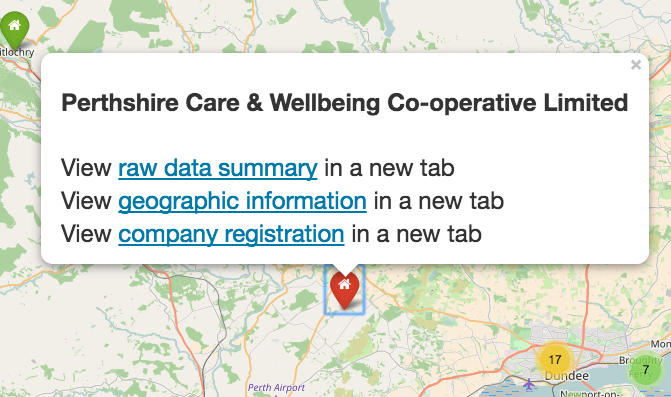
\includegraphics[width=\popupimagewidth]{map-app-popup-screenshot.png}}
  \end{center}
  \begin{itemize}
    \item Web of Documents
    \item Web of Data
  \end{itemize}
}
By clicking on a marker on the map-app, a pop-up will appear, as shown above.
Only the red markers have links to data held by Companies House.

\articleheading{Links}

Some of the links that are displayed in the pop-up are links to two different World Wide Webs: the \textit{Web of Documents} and the \textit{Web of Data}.
The Web of Documents is the one that we are all familiar with; it is the place we inhabit through Web Browsers, and was designed to deliver documents for human beings to read.
The Web of Data shares the same infrastructure (the internet, web servers, etc) as the Web of Documents, but it allows machines to request machine-readable data instead of human-readable documents.

By clicking the \textbf{raw data summary} link, your browser will take you to a page in the Web of Documents that shows data for a co-op. 
That page is identified by a URI (Uniform Resource Identifier) that looks just like a URL (Uniform Resource Locator) you might see in your browser's URL bar. For example:

{\footnotesize \url{http://data.solidarityeconomics.org/id/experimental/test/co-ops-uk/R005512} }

When a web browser requests the web server for that URI, the web server will redirect the browser to a page in the Web of Documents that has the following URL:

{\footnotesize \url{http://data.solidarityeconomics.org/doc/experimental/test/co-ops-uk/R005512.html} }

But, when a machine requests the web server for that same URI, the web server will redirect the machine to data in the Web of Data. 
The machine can request a number of different data formats from the web server.
If the machine requested the Turtle data format, then the web server will redirect it to this URL:

{\footnotesize \url{http://data.solidarityeconomics.org/doc/experimental/test/co-ops-uk/R005512.ttl} }

The machine-readable data in the Turtle format looks like this:

{\footnotesize
\begin{verbatim}
@prefix essglobal: <http://purl.org/solidarityeconomics/experimental/essglobal/vocab/> .
@prefix gr: <http://purl.org/goodrelations/v1#> .
@prefix ospostcode: <http://data.ordnancesurvey.co.uk/id/postcodeunit/> .
@prefix osspatialrelations: <http://data.ordnancesurvey.co.uk/ontology/spatialrelations/> .
@prefix rdf: <http://www.w3.org/1999/02/22-rdf-syntax-ns#> .
@prefix rov: <http://www.w3.org/ns/regorg#> .
@prefix vcard: <http://www.w3.org/2006/vcard/ns#> .
@prefix xsd: <http://www.w3.org/2001/XMLSchema#> .

<http://data.solidarityeconomics.org/id/experimental/test/co-ops-uk/R005512> a essglobal:SSEInitiative;
   gr:name "Pant-yr-Athro Park Management Company";
   essglobal:hasAddress <http://data.solidarityeconomics.org/id/experimental/test/co-ops-uk/R005512Address>;
   essglobal:legalForm <http://purl.org/solidarityeconomics/experimental/essglobal/standard/legal-form/L2>;
   rov:hasRegisteredOrganization <http://business.data.gov.uk/id/company/01113761> .

<http://data.solidarityeconomics.org/id/experimental/test/co-ops-uk/R005512Address> a essglobal:Address;
   osspatialrelations:within ospostcode:SA335AJ;
   vcard:country-name "UK";
   vcard:postal-code "SA33 5AJ" .
\end{verbatim}
}

%\frame[fragile,t]
\frame[t]
{
  \frametitle{Passing links as data}
  \centering
  %\begin{center}
  %\begin{tikzpicture}[scale=.8, show background rectangle, node distance=1cm]
  %\begin{tikzpicture}[remember picture, show background rectangle, node distance=1cm]
  \begin{tikzpicture}[remember picture, node distance=1cm]
    \tikzstyle{every text node part} = [align=center]
    \tikzstyle{obj node} = [ellipse, fill=blue!20]
    \tikzstyle{obj path} = [->, draw=blue!20]
    \tikzstyle{label node} = [draw, text=black]
    \tikzstyle{data node} = [rectangle, fill=green!20]
    \tikzstyle{extdata node} = [rectangle, draw, fill=green!20]
    \tikzstyle{app node} = [rectangle, fill=red!20]
    \tikzstyle{label node} = [midway, auto]
    \tikzstyle{label text} = [align=left]
    \node[obj node] (iseobj) {\underline{Links to other datasets} e.g. \\ {\visible<2->{http://os.gov/postcode/OX10AB}} \\ {\visible<3->{http://ch.gov/company/12345678}}};
    \node[label text, visible on=<1->] (datalabel) [left = of iseobj] {Example \\ data:};
    \node[extdata node, visible on=<2->] (osdata) [below = of iseobj ] {OS data};
    \node[data node] (isedata) [left = of osdata] {Our data};
    \node[extdata node, visible on=<3->] (chdata) [right = of osdata] {CH data};
    \node[label text, visible on=<1->] (datasetlabel) at (isedata-|datalabel) {Datasets:};

    \node[app node, visible on=<4->] (mapapp) [below left = of osdata] {Map};
    \node[app node, visible on=<5->] (nearestapp) [below right = of osdata] {Nearest};
    \node[label text, visible on=<4->] (appslabel) at (mapapp-|datasetlabel) {Apps:};
    \draw[->, visible on=<1->] (isedata) -- (iseobj) node[label node]{contains};
    \draw[->, visible on=<2->] (iseobj) -- (osdata) node[midway, left]{link};
    \draw[->, visible on=<3->] (iseobj) -- (chdata) node[midway, right]{link};
    \draw[<->, visible on=<4>] (mapapp) -- (isedata) node[midway, right]{query};
    \draw[<->, visible on=<4>] (mapapp) -- (osdata) node[midway, right]{query};
    \draw[->, visible on=<5->] (mapapp) -- (nearestapp) node[midway, below]{http://ch.gov/...};
    \draw[<->, visible on=<5->] (nearestapp) -- (osdata) node[midway, left]{query};
    \draw[<->, visible on=<5->] (nearestapp) -- (chdata) node[midway, right]{query};
  \end{tikzpicture}
}

In the picture above ...

\frame
{
  \frametitle{ESSGLOBAL}
  \begin{itemize}
    \item
  \end{itemize}
}
\section{Applications}
\subsection{Example map application}
\subsection{Power of LOD}
\frame
{
  \frametitle{Query across datsets}
  \begin{itemize}
    \item SPARQL demo
  \end{itemize}
}

\section{Conclusions}
\frame
{
  \frametitle{Lessons from re-use}
  \begin{itemize}
    \item Makes the original developers very happy
    \item Great co-operation from original developers
    \item Learn from others
    \item Answers questions you'd not know to ask \texttt{!important;}
    \item Leave things in better shape
  \end{itemize}
}
\frame
{
  \frametitle{LOD Everywhere?}
  \begin{center}
    %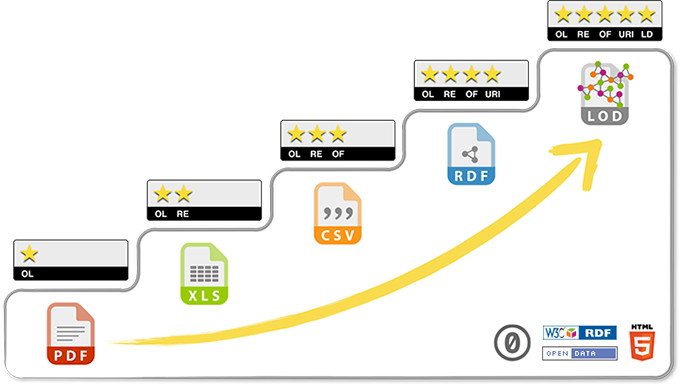
\includegraphics{5-star-steps.png}
    \makebox[\textwidth]{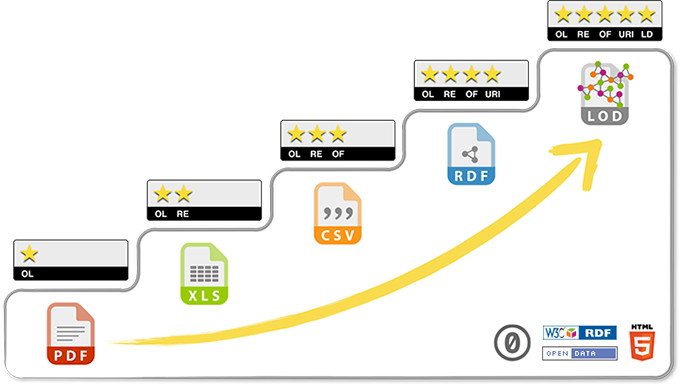
\includegraphics[width=\popupimagewidth]{5-star-steps.png}}
    %\makebox[\textwidth]{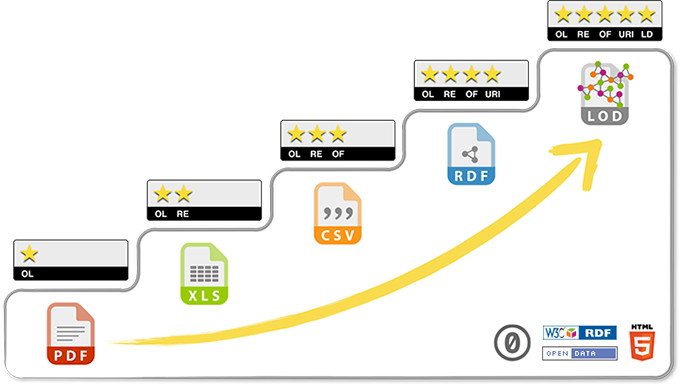
\includegraphics[width=\paperwidth]{5-star-steps.png}}
    %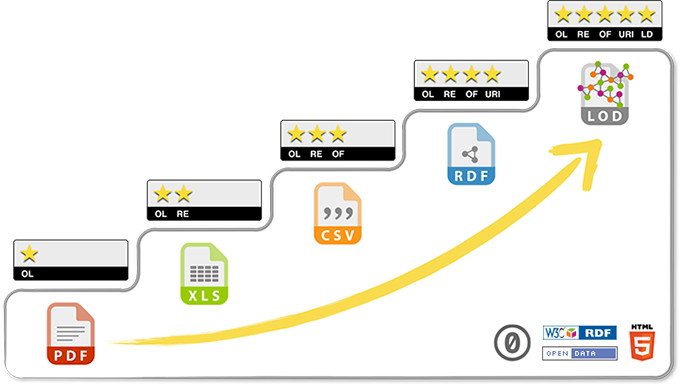
\includegraphics[height=2cm,width=2cm]{5-star-steps.png}
  \end{center}
  \begin{itemize}
    \item \url{http://5stardata.info}
  \end{itemize}
}
\frame
{
  \frametitle{The LOD approach}
  \begin{itemize}
    \item Avoid reinvention of wheels you didn't know existed
    \item Excellent for ``National Grid'' of data
    \item Easliy integrate with other data standards
    \item LOD everywhere? No!

  \end{itemize}
}
\frame
{
  \frametitle{What's next?}
  \begin{itemize}
    \item We can help
    \item How to find out more?
  \end{itemize}
}


\end{document}
